\documentclass[finnish,twoside,censored,tkt,sw-line]{HYthesisML}


% In theses, open new chapters only at right page.
% For other types of documents, may ask "openany" in document.
\PassOptionsToClass{openright,twoside,a4paper}{report}
%\PassOptionsToClass{openany,twoside,a4paper}{report}

\usepackage{csquotes}
%%%%%%%%%%%%%%%%%%%%%%%%%%%%%%%%%%%%%%%%%%%%%%%%%%%%%%%%%
%% REFERENCES
%% Some notes on bibliography usage and options:
%% natbib -> you can use, e.g., \citep{} or \parencite{} for (Einstein, 1905); with APA \cite -> Einstein, 1905 without ()
%% maxcitenames=2 -> only 2 author names in text citations, if more -> et al. is used
%% maxbibnames=99 as no great need to suppress the biliography list in a thesis
%% for more information see biblatex package documentation, e.g., from https://ctan.org/pkg/biblatex

%% Reference style: select one
%% for APA = Harvard style = authoryear -> (Einstein, 1905) use:
% \usepackage[style=authoryear,bibstyle=authoryear,backend=biber,natbib=true,maxnames=99,maxcitenames=2,giveninits=true,uniquename=init]{biblatex}
%% for numeric = Vancouver style -> [1] use:
\usepackage[style=numeric,bibstyle=numeric,backend=biber,natbib=true,maxbibnames=99,giveninits=true,uniquename=init]{biblatex}
%% for alpahbetic -> [Ein05] use:
%\usepackage[style=alphabetic,bibstyle=alphabetic,backend=biber,natbib=true,maxbibnames=99,giveninits=true,uniquename=init]{biblatex}
%

\addbibresource{bibliography.bib}
% in case you want the final delimiter between authors & -> (Einstein & Zweistein, 1905)
% \renewcommand{\finalnamedelim}{ \& }
% List the authors in the Bibilipgraphy as Lastname F, Familyname G,
\DeclareNameAlias{sortname}{family-given}
% remove the punctuation between author names in Bibliography
%\renewcommand{\revsdnamepunct}{ }


%% Block of definitions for fonts and packages for picture management.
%% In some systems, the figure packages may not be happy together.
%% Choose the ones you need.

%\usepackage[utf8]{inputenc} % For UTF8 support, in some systems. Use UTF8 when saving your file.

\usepackage{lmodern}         % Font package, again in some systems.
\usepackage{textcomp}        % Package for special symbols
\usepackage[pdftex]{color, graphicx} % For pdf output and jpg/png graphics
\usepackage{epsfig}
\usepackage{subfigure}
\usepackage[pdftex, plainpages=false]{hyperref} % For hyperlinks and pdf metadata
\usepackage{fancyhdr}        % For nicer page headers
\usepackage{tikz}            % For making vector graphics (hard to learn but powerful)
%\usepackage{wrapfig}        % For nice text-wrapping figures (use at own discretion)
\usepackage{amsmath, amssymb} % For better math
\graphicspath{{../kuvat/}}

\singlespacing{}               %line spacing options; normally use single

\fussy
%\sloppy                      % sloppy and fussy commands can be used to avoid overlong text lines
% if you want to see which lines are too long or have too little stuff, comment out the following lines
% \overfullrule=1mm
% to see more info in the detailed log about under/overfull boxes...
% \showboxbreadth=50
% \showboxdepth=50



%%%%%%%%%%%%%%%%%%%%%%%%%%%%%%%%%%%%%%%%%%%%%%%%%%%%%%%%%
%% STEP 2:
%%%%%%%%%%%%%%%%%%%%%%%%%%%%%%%%%%%%%%%%%%%%%%%%%%%%%%%%%
%% Set up personal information for the title page and the abstract form.
%% Replace parameters with your information.
\title{Koneoppiminen lääkkeiden kehityksessä}

% TM: Contributors to template editors now listed in the beginning of the file in comments
\author{Heikki Pulli}
\date{\today}



% Set supervisors and examiners, use the titles according to the thesis language
% Prof.
% Dr. or in Finnish toht. or tri or FT, TkT, Ph.D. or in Swedish...
\supervisors{Prof.~D.U.~Mind, Dr.~O.~Why}
\examiners{Prof.~D.U.~Mind, Dr.~O.~Why}


\keywords{ulkoasu, tiivistelmä, lähdeluettelo}
\additionalinformation{\translate{\track}}

%% For seminar reports:
%%\additionalinformation{Name of the seminar}

%% Replace classification terms with the ones that match your work. ACM
%% ACM Digital library provides a taxonomy and a tool for classification
%% in computer science. Use 1-3 paths, and use right arrows between the
%% about three levels in the path; each path requires a new line.

\classification{\protect{\ \ \
\  General and reference \(\rightarrow \) Document types  \(\rightarrow \) Surveys and overviews\  \\
\  Applied computing  \(\rightarrow \) Document management and text processing  \(\rightarrow \) Document management \(\rightarrow \) Text editing
}}

%% if you want to quote someone special. You can comment this line out and there will be nothing on the document.
%\quoting{Bachelor's degrees make pretty good placemats if you get them laminated.}{Jeph Jacques}


%% OPTIONAL STEP: Set up properties and metadata for the pdf file that pdfLaTeX makes.
%% Your name, work title, and keywords are recommended.
% \hypersetup{
%     unicode=true,           % to show non-Latin characters in Acrobat’s bookmarks
%     pdftoolbar=true,        % show Acrobat’s toolbar?
%     pdfmenubar=true,        % show Acrobat’s menu?
%     pdffitwindow=false,     % window fit to page when opened
%     pdfstartview={FitH},    % fits the width of the page to the window
%     pdftitle={},            % title
%     pdfauthor={},           % author
%     pdfsubject={},          % subject of the document
%     pdfcreator={},          % creator of the document
%     pdfproducer={pdfLaTeX}, % producer of the document
%     pdfkeywords={something} {something else}, % list of keywords for
%     pdfnewwindow=true,      % links in new window
%     colorlinks=true,        % false: boxed links; true: colored links
%     linkcolor=black,        % color of internal links
%     citecolor=red,        % color of links to bibliography
%     filecolor=magenta,      % color of file links
%     urlcolor=cyan           % color of external links
% }

%%-----------------------------------------------------------------------------------

\begin{document}

% Generate title page.
\maketitle


%%%%%%%%%%%%%%%%%%%%%%%%%%%%%%%%%%%%%%%%%%%%%%%%%%%%%%%%%
%% STEP 3:
%%%%%%%%%%%%%%%%%%%%%%%%%%%%%%%%%%%%%%%%%%%%%%%%%%%%%%%%%
%% Write your abstract to be positioned here.
%% You can make several abstract pages (if you want it in different languages),
%% but you should also then redefine some of the above parameters in the proper
%% language as well, in between the abstract definitions.

\begin{abstract}

    Tämä dokumentti on tarkoitettu Helsingin yliopiston tietojenkäsittelytieteen osaston opin\-näyt\-teiden ja harjoitustöiden ulkoasun ohjeeksi ja mallipohjaksi. Ohje soveltuu kanditutkielmiin, ohjelmistotuotantoprojekteihin, seminaareihin ja maisterintutkielmiin. Tämän ohjeen lisäksi on seurattava niitä ohjeita, jotka opastavat valitsemaan kuhunkin osioon tieteellisesti kiinnostavaa, syvällisesti pohdittua sisältöä.


    Työn aihe luokitellaan
    ACM Computing Classification System (CCS) mukaisesti,
    ks.\ \url{https://www.acm.org/about-acm/class},
    käyttäen komentoa \verb+\classification{}+.
    Käytä muutamaa termipolkua (1--3), jotka alkavat juuritermistä ja joissa polun tarkentuvat luokat erotetaan toisistaan oikealle osoittavalla nuolella.

\end{abstract}

% \begin{otherlanguage}{english}
%     \begin{abstract}
%         Use this otherlanguage environment to write your abstract in another language if needed.

%         Topics are classified according to the ACM Computing Classification System
%         (CCS), see
%         \url{https://www.acm.org/about-acm/class}:
%         check command \verb+\classification{}+. A small set of paths (1--3) should be used, starting from any top nodes
%         referred to bu the root term CCS leading to the leaf nodes. The elements
%         in the path are separated by right arrow, and emphasis of each element individually can be indicated
%         by the use of bold face for high importance or italics for intermediate
%         level. The combination of individual boldface terms may give the reader
%         additional insight.
%     \end{abstract}
% \end{otherlanguage}

% Place ToC
\newpage
\mytableofcontents{}
\mainmatter{}

%%%%%%%%%%%%%%%%%%%%%%%%%%%%%%%%%%%%%%%%%%%%%%%%%%%%%%%%%
%% STEP 4: Write the thesis.
%%%%%%%%%%%%%%%%%%%%%%%%%%%%%%%%%%%%%%%%%%%%%%%%%%%%%%%%%
%% Your actual text starts here. You shouldn't mess with the code above the line except
%% to change the parameters. Removing the abstract and ToC commands will mess up stuff.
%%
%% You may wish to include material to avoid browsing the definitions
%% above. Command \include{file} includes the file of name file.tex.
%% As a side effect, subsequent inclusions may force a page break.

% BSc instructions
%\include{bsc_finnish_contents}
%\include{bsc_english_contents}
% MSc instructions
%\include{msc_finnish_contents}
% \include{msc_english_contents}

%%%%%%%%%%%%%%%%%%%%%%%%%%%%%%%%%%%%%%%%%%%%%%%%%%%%%%%%%

\chapter{Johdanto}

Uusien lääkkeiden kehittäminen on pitkä ja kallis prosessi.
Tähän kuuluu useita vaiheita ja eri vaiheet vievät eri määrän rahaa ja aikaa.
Vaiheet ovat sairauden aiheuttajan tunnistaminen, aiheuttajaan vaikuttavan lääkkeen tunnistaminen, lääkkeen optimointi, lääkkeen ominaisuuksien analysointi ja kliiniset testit.
Näiden jälkeen lääke joko hyväksytään myyntiin tai ei.
Vaiheet ovat tavallisesti vieneet 10--12 vuotta ja kaikkien vaiheiden jälkeen työn hinnaksi on voinut muodostua 1--3 miljardia dollaria~\cite{EkinsSean2019Emlf}.

Vaiheiden pitkän keston ja korkean hinnan takia tutkijat ja lääkealan yritykset ovatkin alkaneet tutkia mahdollisia keinoja, jotka nopeuttaisivat tai halventaisivat tätä lääkekehityksen prosessia.
Koneoppimismallit ovat nousseet houkuttelevaksi vaihtoehdoksi prosessin nopeuttamiseksi.
Yritykset ovatkin alkaneet selvittää, kuinka eri koneoppimismalleja voidaan hyödyntää nopeuttamaan lääketutkimuksen suurimpia pullonkauloja~\cite{EkinsSean2019Emlf}.
Viimeisen kymmenen vuoden aikana saatavilla olevan laadukkaan datan määrä on kasvanut merkittävästi ja samalla on kehitetty uusia tehokkaampia koneoppimismalleja, joita voidaan hyödyntää lääketutkimuksessa.
Koneoppimismallien avulla voidaan esimerkiksi karsia kaikista harkinnasta olevista lääkkeistä lupaavimmat kandidaatit, joilla on mahdollisuus päästä testeistä läpi tuotantoon.
Koneoppimismalleja voidaan myös hyödyntää aivan uusien lääkkeeksi sopivien yhdisteiden etsinnässä.
Tähän tarkoitukseen kehitetyt koneoppimismallit kykenevät etsimään lääkkeitä, joilla on halutut lääkkeelliset ja fysikaaliset ominaisuudet~\cite{VamathevanJessica2019Aoml}.
Kehitetyt mallit ovatkin näyttäneet, että koneoppimismallit ovat tehokkaita työkaluja, joita voidaan hyödyntää kaikissa lääketutkimuksen eri vaiheissa.

Tässä tekstissä paneudutaan syvemmin koneoppimismalleihin, joita käytetään uusien lääkkeiden tunnistamiseen ja näiden tunnistettujen lääkkeiden syntetisoinnin suunnitteluun.

Ensimmäisessä kappaleessa tutustutaan eri datatyyppeihin, joita käytetään koneoppimismallien kouluttamisessa.
Näiden ymmärtäminen auttaa hahmottamaan myöhemmin tekstissä selitettävien eri mallien toimintaperiaatteita.

Toisessa kappaleessa käydään läpi, kuinka uusia lääkkeitä löydetään.
Kappaleessa kerrotaan virtualisesta seulonnasta (Virtual screening), mitä sillä tarkoitetaan ja kuinka sitä hyödynnetään.
Lisäksi toisessa kappaleessa käydään läpi yhden koneoopimismallin toimintaa.
Tämä koneoppimismalli keskittyy uusien lääkkeiden löytämiseen.

Kolmannessa kappaleessa käsitellään yhdisteiden syntetisointia.
Kappaleessa kerrotaan, mikä tekee yhdisteiden syntetisoinnista hankalaa ja mitä ratkaisuja tähän on kehitetty.
Kappale myös kertoo retrosyntetisoinnista, CASP -menetelmistä (\textbf{Computer Aided Synthesis Planning}) ja kuinka nämä liittyvät toisiinsa.
Lisäksi kappaleessa käydään läpi kahden eri koneoppimismallin toimintaa, jotka on kehitetty auttamaan eri yhdisteiden syntetisoinnissa.

Neljäs kappale käsittelee, kuinka koneoppimista tullaan käyttämään tulevaisuuden lääkekehityksessä ja tutkimisessa.
Kappale kertoo, kuinka koneoppiminen tulee enenemissä määrin muuttamaan lääkekehityksen prosessia.

\chapter{Kemiallinen data}

Tässä kappaleessa käydään pintapuolisesti läpi, minkälaista dataa käytetään mallien kouluttamiseen.
Kappaleessa keskitytään datatyyppeihin, joita käytetään malleissa, joiden toimintaa tullaan avaamaan tämän tekstin muissa osissa.
Mallit, joiden toimintaa avataan, käyttävät datatyyppejä, joilla kuvataan pienyhdisteitä.
Tämän takia kappaleessa keskitytään pieniäyhdisteitä kuvaaviin datatyyppeihin.
Kappaleessa käydään läpi SMILES ja SMARTS datatyypit, mihin niitä käytetään ja kuinka ne eroavat toisistaan.
Lisäksi kappaleessa kerrotaan ominaisuusvektoreista, kuinka niitä käytetään ja missä tilanteissa.

\section{SMILES, SMARTS ja SMIRKS}

SMILES (Simplified Molecular Input Line Entry System) on David Weiningerin vuonna 1988 kehittämä tapa kuvata molekyylejä ja yksinkertaisia yhdisteitä~\cite{WeiningerSMILES}.
Se kuvaa yhdisteen yhdellä rivillä käyttäen ASCII -merkistöä.
Tämän takia se on tietokoneen nopea lukea ja kemistin helppo ymmärtää.

\begin{figure}
    \centering
    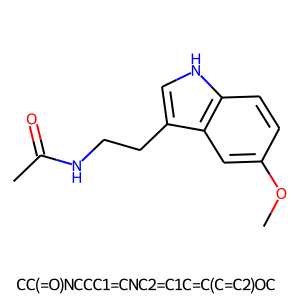
\includegraphics[width=8cm, height=8cm]{melatonin-smiles.png}
    \caption{Melatoniini yhdiste, kuinka se kuvataan graaffina ja SMILES -merkijonona.
        Kuva on tuotettu hyödyntämällä RDKit -kirjastoa.}
    {~\cite{ShinBonggun}}
\end{figure}

SMARTS on puolestaan SMILES:ista jatkettu tapa kuvata yhdisteitä.
Se mahdollistaa yhdisteiden sisäisten rakenteiden määrittämisen.
Tämän takia kaikki SMILES -merkkijonoiksi kelpaavat merkkijonot ovat myös kelpoja SMARTS -merkkijonoja.

SMIRKS on edelleen jatkokehitetty tapa kuvata yhdisteiden välisiä reaktioita ASCII -merkistöllä.

\section{Ominaisuusvektorit}

\chapter{Uusien lääkkeiden löytäminen}

% Miksi uusien lääkkeiden löytäminen on vaikeaa?~\cite{EkinsSean2019Emlf}

Tässä kappaleessa kerrotaan, mitä asioita liittyy lääkkeiden löytämiseen.
Lisäksi kappaleessa kerrotaan, mitä on virtuaalinen seulonta ja kuinka sitä hyödynnetään lääkkeiden löytämisessä.
Kappaleessa myös käydään läpi yhden koneoppimismallin toimintaperiaate.
Kyseinen koneoppimismalli luo uusia lääkkeitä perustuen ominaisuusvektoreihin.

\section{Lääkkeiden löytäminen}

Yksi ensimmäisistä lääkekehityksen osa-alueista on uusien lääkkeiksi kelpaavien yhdisteiden löytäminen joko uusiin tai jo tunnettuihin tauteihin~\cite{EkinsSean2019Emlf}.
Lääkeyhdisteiden löytäminen on kuitenkin ollut tavallisesti hidas prosessi ja uuden toimivan yhdisteen löytäminen on kestänyt useita vuosia.

Viimeisimmän kymmenen vuoden aikana saatavilla olevan datan määrä on kasvannut merkittävästi kehitettyjen tietopankkien takia~\cite{EkinsSean2019Emlf}.
Näitä ovat esimerkiksi PubChem ja ChEMBL.\
Lisääntynyt datan määrä on täten mahdollistanut lääkkeiden löytämisen nopeuttamisen koneoppimismallien avulla.

Popovan et al.\ tutkimusryhmä on kehittänyt mallin, joka ehdottaa uutta yhdistettä perustuen mallin syötteenä saamaan ominaisuusvektoriin~\cite{PopovaMariya2018Drlf}.

\section{Virtuaalinen seulonta}

Kemiallisten yhdisteiden avaruudella tarkoitetaan kaikkien uniikkien yhdisteiden lukumäärää.
On arvioitu, että erilaisia kemiallisia yhdisteitä, jotka voivat esiintyä huoneenlämmössä ja nesteessä, voi olla välillä \(10^{18} - 10^{180}\)~\cite{SotrifferChristoph2011VSPC}.
Yhdisteet, jotka täyttävät lääkkeeltä vaaditut kriteerit, on puolestaan arvioitu olevan noin \(10^{60}\)~\cite{SotrifferChristoph2011VSPC}.
Erillaisten yhdisteiden suuri lukumäärä itsessään esittää tarpeen tehokkaille algoritmeille ja menetelmille, jotka auttavat karsimaan tästä suuresta määrästä kemiallisia yhdisteitä vain lupaavimmat.

Virtuaalinen seulonta (Virtual Screning, VS) on suosittu lähestymistapa uusien lääkkeiden löytämiseksi.
VS käsittää joukon menetelmiä, joissa tietokoneita hyväksi käyttäen karsitaan yhdisteiden avaruudesta vain tietyt kriteerit täyttävät yhdisteet~\cite{SotrifferChristoph2011VSPC}.
Yhdisteiden karsimiseen käytetään ohjelmistoja, joissa toteutetut algoritmit suorittavat seulontaa.
Koneoppimismenetelmiä voidaan myös käyttää virtuaalisessa seulonnassa.
VS:än avulla löydettyjä yhdisteitä voidaan sitten jatkotutkia ja edelleen kehittää lääkkeiksi.

\section{Kehitettyjä koneoppimismalleja}

Käydään seuraavaksi läpi yhden toteutetun koneoppimismallin toimintaperiaate.
Kyseinen malli etsii uusia lääkkeitä käyttämällä hyödyksi sille annettua prototyyppiyhdistettä, prototyypin kemiallisia ominaisuuksia ja uudelta lääkkeeltä haluttuja kemiallisia ominaisuuksia.
Kemialliset ominaisuudet on koodattu ominaisuusvektoreihin.

\subsection{CMG}

CMG (Controlled molecule generator) on koneoppimismalli, joka etsii uusia molekyylejä, jotka perustuvat syötteenä annettuun molekyyliin ja joilla on ennalta määritellyt halutut ominaisuudet~\cite{ShinBonggun}.
Se eroaa aikaisemmin kehitetyistä malleista siten, että se pystyy optimoimaan annetun molekyylin useampaa ominaisuutta.
Aikaisemmat mallit ovat pystyneet optimoimaan vain yhtä molekyylin ominaisuutta.

CMG:n kehittäjät lähestyvät molekyylin ominaisuuksien optimointiongelmaa merkkijonojen käännös -ja luontiongelmana.
CMG:lle opetetaan, kuinka syötteenä annettu molekyylimerkkijono käännetään molekyylimerkkijonoksi, jolla on lähimpänä haluttuja ominaisuuksia olevat ominaisuudet.
CMG tulkitsee ensin annetut merkkijonot hyödyntäen DN:ää (deep network) jonka jälkeen se luo uusia molekyyliyhdisteitä hyödyntäen tätä tulkintaa ja haluttua ominaisuusvektoria.
Koska ominaisuudet annetaan vektorina, niin CMG pystyy optimoimaan useampaa ominaisuutta.
CMG lisäksi hyödyntää ennalta koulutettuja rajoiteverkkoja (constraint network, CN), jolloin vältytään luomasta mahdottomia yhdisteitä.
CMG -malli käyttää näitä verkkoja hyödyksi käyttämällä muokattua Beam Search -algoritmia.

% (Taustatietoa muista aiheista/malleista, joita on hyödynnetty CMG:ssä\dots)

CMG -malli muodostuu kolmesta verkosta, joista kaksi toimivat rajoiteverkkoina.
Ensimmäinen verkko on MTN (\textbf{Molecule Translation Network}) ja rajoiteverkot ovat PPN (\textbf{Property Prediction Network}) ja SPN (\textbf{Similarity Prediction Network}).

MTN -verkko perustuu aikaisemmin kehitettyyn  The Transformer -malliin~\cite{TheTransformer}.
MTN eroaa Transformer -mallista kahdella tavalla.
Toisin kuin Transformer -malli, joka käsittelee sanoja ja niistä muodostettuja lauseita, MTN -verkko käsittelee yksittäisiä merkkejä ja niistä muodostettuja molekyylejä.
Lisäksi MTN:än piilotettuun kerrokseen on lisätty tietoa kemiallissista ominaisuuksista.
MTN:än kustannusfunktio on muotoa \[\mathcal{L} (\theta_T;X,p_x,p_y) = -\frac{1}{N}\frac{1}{M}\sum_{n \in N}\sum_{i \in M}\sum_{v \in V}y_v,j,n \cdot \log(\hat{y}_v,j,n).\]

PPN -verkko ottaa syötteenä ennustetun molekyylin merkkijonon (\(y_i\)).
Tämä merkkijono muunnetaan piilotetuiksi vektoreiksi (Parempi termi?) hyödyntäen Long short-term memory (LSTM) -kerrosta.
LSTM -kerros muodostaa vektoreita oikealta vasemmalle ja vasemmalta oikealle suunnassa, ja näistä vektoreista valitaan molempien suuntien viimeiset vektorit.
Nämä vektorit yhdistetään ja yhdistevektori syötetään täysin yhdistetylle neuroverkolle.
Tämä verkko sisältää kaksi piilotettua tasoa.

SPN ottaa syötteenä ennustetun molekyylin merkkijonon (\(y_i\)) ja alkuperäisen molekyylin merkkijonon (\(x_i\)).
Nämä merkkijonot syötetään kahdelle eri LSTM -tasolle, toinen käsittelee alkuperäisen molekyylin merkkijonot ja toinen ennustetun molekyylin merkkijonot.
Nämä LSTM -kerrokset tomivat samalla periaatteella kuin PPN:ässä ja palauttavat näin ollen neljä eri vektoria.
Nämä vektorit yhdistetään ja tämä yhdistevektori annetaan täysin yhdistetylle verkolle, joka sisältää kaksi piilotettua tasoa.

\begin{figure}
    \centering
    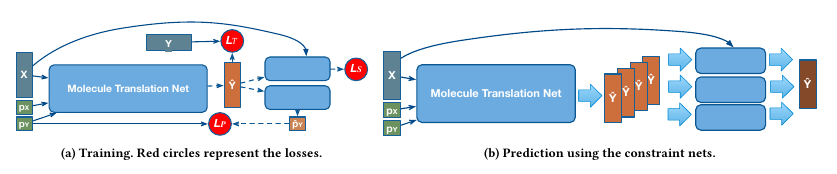
\includegraphics[width=\textwidth]{CMG-fig.png}
    \caption{CMG:n toiminta periaate kuvattuna}
    {~\cite{ShinBonggun}}
\end{figure}

Data, jolla mallit koulutetaan, on peräisin ZINC ja DRD2 dataseteistä. (Kuka hallinnoi?)
Data sisältää kaiken kaikkiaan 257 565 molekyyliä, joista luodaan pareja.
Parit muodostetaan siten, että kahden molekyylin välinen samanlaisuusluku on yli 0.4. (Miten lasketaan?)
Näitä pareja \((X,Y)\) muodostetaan kaiken kaikkiaan 10 827 615 kappaletta.
Lisäksi kaikille molekyyleille lasketaan niiden eri kemiallisten ominaisuuksien arvot, jotka ovat PlogP, QED ja DRD2.
Nämä kuvaavat eri haluttuja ominaisuuksia, joita lääkkeiltä halutaan.

PPN koulutetaan käyttäen 257 565 eri molekyyliä.
nämä molekyylit jaetaan satunnanvaraisella valinnalla koulutus -ja testiryhmiin suhteella 8:2.

SPN kouluttamiseen käytetään osajoukkoa 10 827 615 eri parista.
Tästä määrästä valitaan kymmenen prosentin osajoukko, joka on kaiken kaikkiaan 997 773 molekyylin suuruinen.
Tämä joukko jaetaan samalla tavalla koulutus ja testi ryhmiin kuin PPN:ässä.

\subsubsection{CMG:n suorituskyky}

\chapter{Uusien lääkkeiden syntetisointi}

Tässä kappaleessa käydään läpi, miten lääkkeiden syntetisoinnin suunnittelua voidaan tehdä koneoppimismallien avulla.
Kappaleessa keskitytään syntetisointiin retrosyntetisoinnin avulla.
Kappaleessa kerrotaan, mikä tekee yhdisteen retrosyntetisoinnista vaikeaa ja kuinka sitä voidaan tehostaa eri koneoppimismallien avulla.
Kappaleessa käydään läpi kahden koneoppimismallin toimintaa, jotka suorittavat halutun yhdisteen retrosyntetisointia.

\section{Yhdisteiden syntetisointi}

Yhdisteen syntetisoinnin suunnittelulla tarkoitetaan prosessia, jossa määritellään, kuinka haluttu yhdiste voidaan tuottaa synteettisesti saatavilla olevista lähtöaineista~\cite{ColeyConnorW2018MLiC}.
Retrosynteesianalyysillä tarkoitetaan puolestaan menetelmää, jonka avulla löydetään halutun yhdisteen tuottamiseen tarvittavat lähtöaineet.
Retrosynteesi toimii siis toiseen suuntaan kuin syntetisointi.
Retrosynteesissä yhdiste pilkotaan rekursiivisesti pienempiin lähtöaineisiin kunnes jäljellä on vain saatavilla olevia lähtöaineita.

Tavallisesti yhdisteen retrosyntetisointi on vaatinut suorittavalta kemistiltä usean vuoden kokemusta ja tietoa saatavilla olevista lähtöaineista ja eri reaktioista.
Tätä on pyritty automatisoimaan eri CASP -menetelmien avulla (Computer-Aided Synthesis Planning).
Ensimmäiset CASP -menetelmät perustuivat heuristisiin algoritmeihin, joissa kemistit käsin koodasivat, miten eri lähtöaineet reagoivat keskenään ja mikä on reaktion lopputuote.
Tämä on kuitenkin osoittautunut toivottomaksi yritykseksi massiivisen datan määrän takia.

Kehitys koneoppimismenetelmissä on kuitenkin tarjonnut uuden lähestymistavan CASP -menetelmien kehitykseen.
Sen sijaan, että kemistit kehittäisivät heuristisia malleja, uudet koneoppimismallit koulutetaan saatavilla olevan datan avulla.
Tämä on todettu merkittävästi enemmän toteutettavaksi lähestymistavaksi.

Koneoppimismallien käyttö ja koulutus ei ole kuitenkaan täysin ongelmaton lähestymistapa.
Ongelmaan liittyvää dataa ei välttämättä ole saatavilla ja datan hankkiminen voi olla kallista.
Tätä varten on kehitetty tietopankkeja, jotka sisältävät suuria määriä dataa tietystä aiheesta, esim. Reaxys kemiallisesista reaktioista.

\section{Lääkkeen retrosyntetisoinnin haastavuus}

Retrosyntetisoinnin tekee hankalaksi se, että yhdiste voidaan muodostaa sadoilla tai tuhansilla eri tavoilla.
Tämä ongelma toistuu rekursiivisesti, kun yhdiste pilkotaan yhdisteisiin, jotka keskenään reagoidessa muodostavat alkuperäisen yhdisteen.
Pienille ja yksinkertaisille yhdisteille tämä vaihtoehtoavaruus on pienempi, mutta yhdisteen koon kasvaessa eri tapojen määrä muodostaa haluttu yhdiste kasvaa eksponentiaalisesti.

Tästä johtuen prosessia yleistäville koneoppimismalleille on suuri.

% Miksi lääkkeiden retrosyntetisointi on hankalaa~\cite{ButlerKeithT2018Mlfm,deAlmeidaA.Filipa2019Socd}?
\begin{figure}
    \centering
    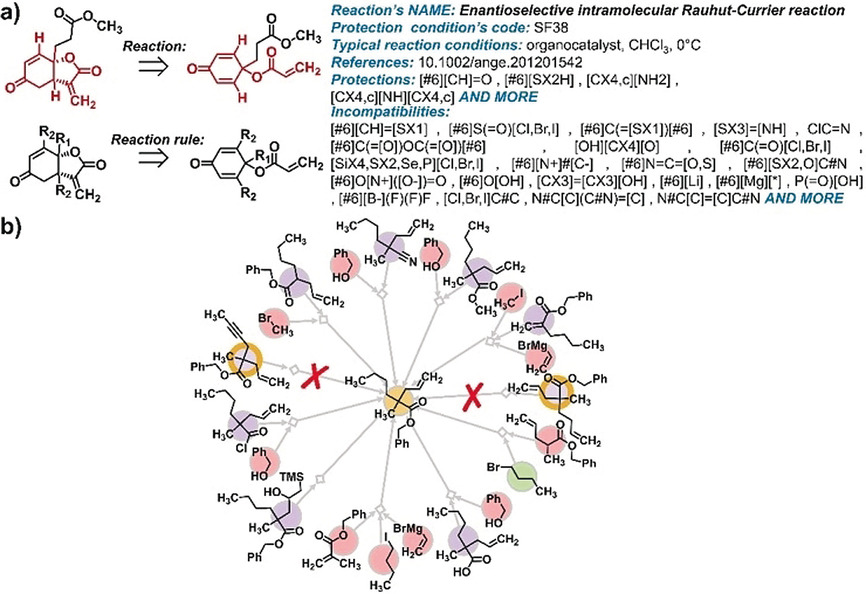
\includegraphics[width=\textwidth]{retrosynthesis.jpg}
    \caption{(a) esimerkki reaktiosäännöstä, (b) esimerkki mahdollisista reaktioista, kuinka voidaan luoda haluttu yhdiste (keskellä).
        Kuvaa on yksinkertaistettu ja se sisältää vain yksitoista mahdollista reaktiota, jotka tuottavat halutun yhdisteen.
        Värikoodaukset tarkoittavat: Keltainen --- haluttu yhdiste, Punainen --- saatavilla oleva yhdiste, Vihreä --- kirjallisuudesta tunnettu yhdiste, liila --- tuntematon yhdiste}
    {~\cite{ExpertKnowledgeRetorsynthesis}}
\end{figure}

\section{Kehitettyjä apuvälineitä}

Seuraavissa kappaleissa vataan kahden kehitetyn koneoppimismallin toimintaa.
Nämä mallit ovat toteutettu suorittaman retrosynteesiä, mutta niiden toimintaperiaate perustuu eri lähestymistapaan.
3N-MCTS -mallin toimintaperiaate perustuu täysin oppimiseen datasta, kun taas ICHO -malli hyödyntää myös ammattikemistien luomia heuristisiasääntöjä.

\subsection{3N-MCTS}

3N-MCTS on koneoppimismalli, jonka on kehittänyt Marwin et al.
Se etsii retrosynteesipolkuja yksinkertaisempiin ja saatavilla oleviin lähtöaineisiin~\cite{SeglerMarwinHS2018Pcsw}.
Kun retrosynteesipolku on varmennettu ja todettu toimivaksi, niin syötteenä annettu yhdiste on mahdollista syntetisoida laboratoriossa.

3N-MCTS -malli muodostuu kolmesta eri koneoppimismallista ja Monte Carlo -puuhakualgoritmista (\textbf{Monte Carlo Tree Search, MCTS}).
Neuroverkot on koulutettu avustamaan puuhakualgoritmia etenemään järkevimpään suuntaan, kun haku algoritmi etsii syntetisointipolkuja ja tarkistamaan, onko ehdotettu reaktio mahdollinen kyseiselle molekyylille.

Neuroverkot ovat hakupuun laajentumisen suuntaa ohjaava verkko (\textbf{Expansion policy network, EPN}), MCTS:än rollout toimintoa tukeva Rollout -verkko (\textbf{Rollout policy network, RPN}) ja verkko, joka tarkistaa, onko syntetisointi polku toteutettavissa (\textbf{In-scope filter network, IFN}).

Data, jolla neuroverkot koulutetaan, on peräisin Reaxys -tietokannasta.
Reaxyksen omistaa Elsevier kustantamo.
Reaxys -tietokannan sisältämä data koostuu muunnossäännöistä (\textbf{transformation rule}), jotka kertovat, mitkä lähtöaineet reagoivat keskenään, mikä reaktio on kysessä ja mikä on reaktion lopputuote.
Näitä sääntöjä käytetään mallien kouluttamiseen.
Tietokanta sisältää yli 12.4 miljoonaa sääntöä.
Mallien kouluttamiseen käytetyt säännöt sisältävät vain yksivaiheisia kemiallisia reaktioita ja reaktiossa on mukana vain yhdestä kolmeen lähtötuotetta.
Eri mallien kouluttamiseen käytetään eri kriteerein suodatettua dataa tietokannasta.
Kaikki koneoppimismallit koulutetaan käyttämällä ADAM -optimoijaa.
ADAM -optimoija hyödyntää AdaGrad:in ja RMSProp:in toiminnallisuutta~\cite{kingma2017adam}.

\subsubsection{3N-MCTS toimintamalli}

\begin{figure}
    \centering
    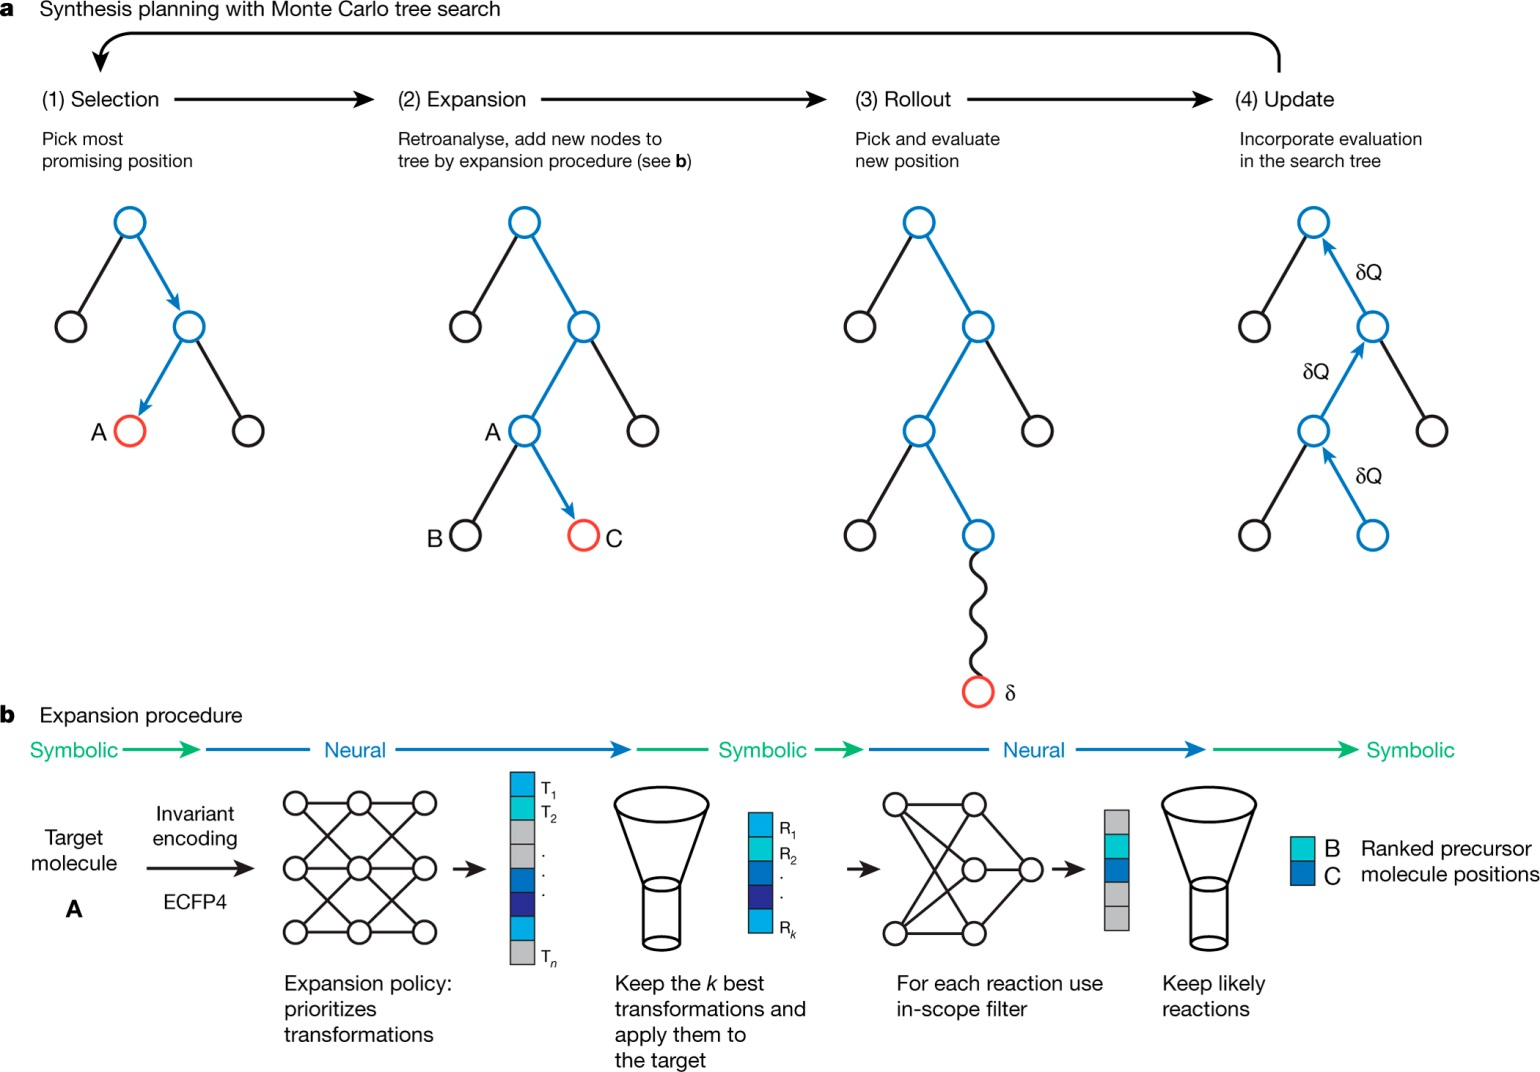
\includegraphics[width=\textwidth]{3N-MCTS-fig.jpg}
    \caption{3N-MCTS:än toiminta periaate kuvattuna}
    {~\cite{SeglerMarwinHS2018Pcsw}}
\end{figure}

3N-MCTS -mallin IFN ja EPN on kehitetty toimimaan yhdessä.
Tutkittaessa puun tilaa \(S_i\) (selitä Si vaihe) jokainen molekyyli syötetään EPN:älle ja se tulostaa, mitkä säännöt voivat muodostaa annetun yhdisteen ja näin ollen myös mitkä lähtöaineet voivat muodostaa annetun yhdisteen.
Nämä säännöt syötetään IFN:älle, joka suodattaa valituista reaktioista toteutettavissa olevat vaihtoehdot.
Tämän jälkeen algoritmissa iteroidaan neljää vaihetta, jotka muodostavat lopullisen puun.

(1) Ensimmäisessä vaiheessa algoritmi valitsee seuraavan lupaavimman tilan puusta kunnes puun lehti on saavutettu.
Jos lehdessä käydään ensimmäisen kerran valintavaiheen aikana, niin lehti arvostellaan simuloimalla hakualgoritmia \(d\) askelta eteenpäin samalla muodostaen synteesipolkua (rollout).
Jos lehdessä käydään useamman kuin yhden kerran valintavaiheen aikana, niin mahdolliset säännöt, jotka muodostavat lehden, tutkitaan ja lisätään lehden lapsiksi (expansion).

(2) Toisessa vaiheessa lupaavien tilojen lapset tutkitaan.
Tällöin etsitään lupaavimmat säännöt, jotka muodostavat kyseisessä tilassa olevan yhdisteen.

(3) Kolmannessa vaiheessa tarkistetaan lehden tila.
Jos lehti on `todistetusti toimiva', niin algoritmi palauttaa luvun suuremman kuin yksi, jolloin lehteä suositellaan käytettävän synteesipolussa.
Muussa tapauksessa lehdelle suoritetaan rollout, jolloin RPN antaa rekursiivisesti uusia sääntöjä niin kauan, kunnes lehti on pilkottu lähtöaineisiin tai kunnes suurin sallittu syvyys \(d\) on saavutettu.

(4) Viimeisessä vaiheessa lehtien arvot päivitetään.
Jos lähtöaineet löydetään rolloutin aikana, niin lehti saa palkonnoksi arvon 1.
Jos Kaikkia lähtöaineita ei löydetty, niin lehdelle annetaan osittainen palkinto.
Jos yhtään lähtöainetta ei löytynyt, niin lehti saa arvon -1.

Saattaa kuitenkin olla, että synteesipolkua ei voida luoda.
Joko synteesipolun tutkimiseen menee liian kauan aikaa tai synteesipolku sisältää liian monta vaihetta yhdisteen syntetisoimiseen.


\subsubsection{Expansion policy netwrok}

\begin{figure}
    \centering
    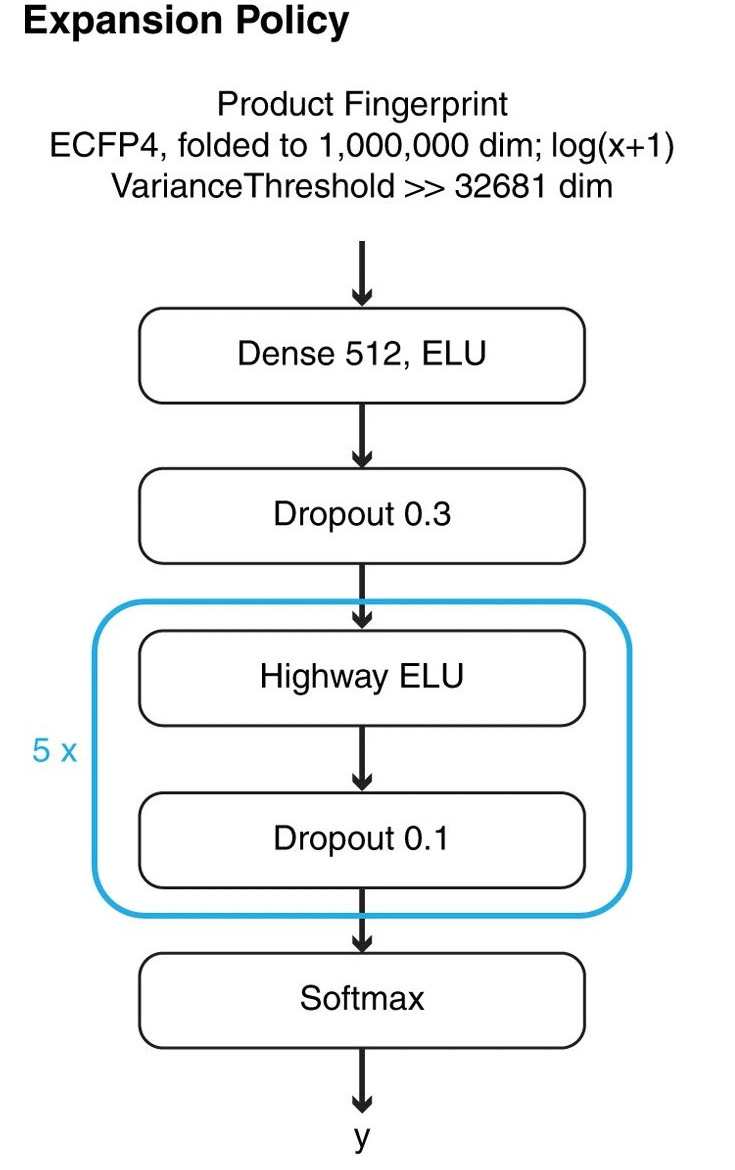
\includegraphics[]{expansion-policy.jpg}
    \caption{Kuvassa expansion policy -neuroverkon rakenne.}
    {~\cite{SeglerMarwinHS2018Pcsw}}
\end{figure}

EPN muodostuu täysin kytketystä tasosta ja viidestä highway -tasosta.
Molemmissa tasoissa on käytetty aktivointifunktiona ELU -funktiota (\textbf{Exponential Linear Unit}).
Täysin kytketyssä tasossa suoritetaan dropout, jonka jälkeen vain 0.3 ensimmäisen tason solmujen tuloksista otetaan huomioon seuraavalla tasolla.
Tämän jälkeen jokaisen highway -tason jälkeen suoritetaan 0.1 dropout.
EPN -verkon viimeinen taso on softmax, joka palauttaa todennäköisyysjakauman.
Tämä jakauma kertoo kuinka todennäköisesti muunnossääntö \emph{a} muodostaa tuotteen \emph{m}.

EPN -verkon kouluttamiseen valittiin datasta vain reaktiokeskus.
Datasta suodatettiin pois sellaiset säännöt, jotka ilmenivät datassa alle kolme kertaa ennen vuotta 2015.
Lopullinen reaktiomäärä, jolla EPN koulutettiin, oli 301 671 reaktiota.

\subsubsection{Rollout policy network}

\begin{figure}
    \centering
    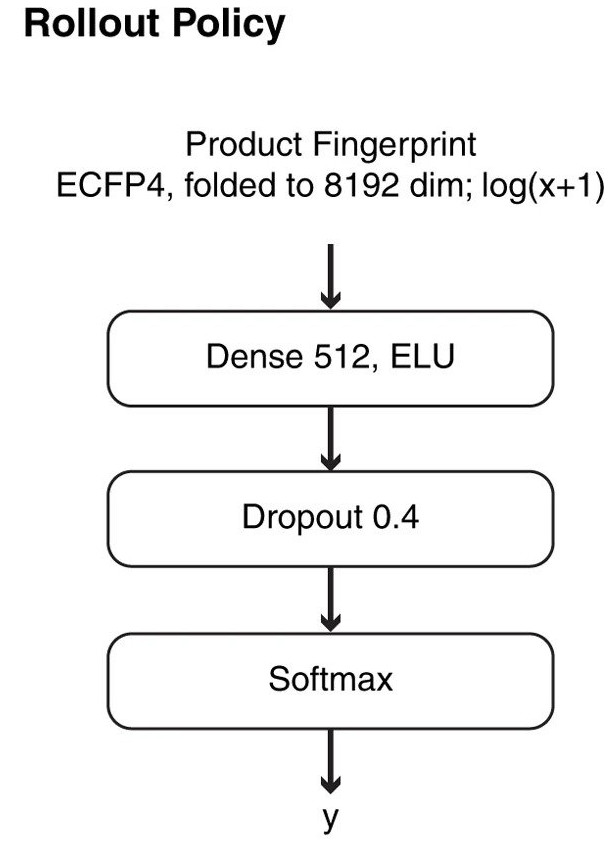
\includegraphics[]{rollout-policy.jpg}
    \caption{Kuvassa Rollout policy -neuroverkon rakenne.}
    {~\cite{SeglerMarwinHS2018Pcsw}}
\end{figure}

% RPN on neuroverkko, jossa on yksi piilotettu kerros. RPN koulutettiin samalla tavalla kuin EPN.\@

RPN muodostuu yhdestä täysin kytketystä tasosta.
Samalla tavalla kuin EPN, RPN käyttää myös ELU -funktiota aktivointifunktiona.
RPN -verkon viimeinen taso on myös softmax, joka palauttaa todennäköisyysjakauman.

RPN -verkon kouluttamiseen valittiin datasta vain reaktiossa muuttuneet atomit ja liitokset (reaktiokeskus) ja lähimmät vierekkäiset atomit.
Datasta suodatettiin pois sellaiset säännöt, jotka ilmaantuivat alle 50 kertaa ennen vuotta 2015.
Lopullinen reaktiomäärä, jolla RPN koulutettiin, oli 17 134 reaktiota.

\subsubsection{In-scope filter network}

\begin{figure}
    \centering
    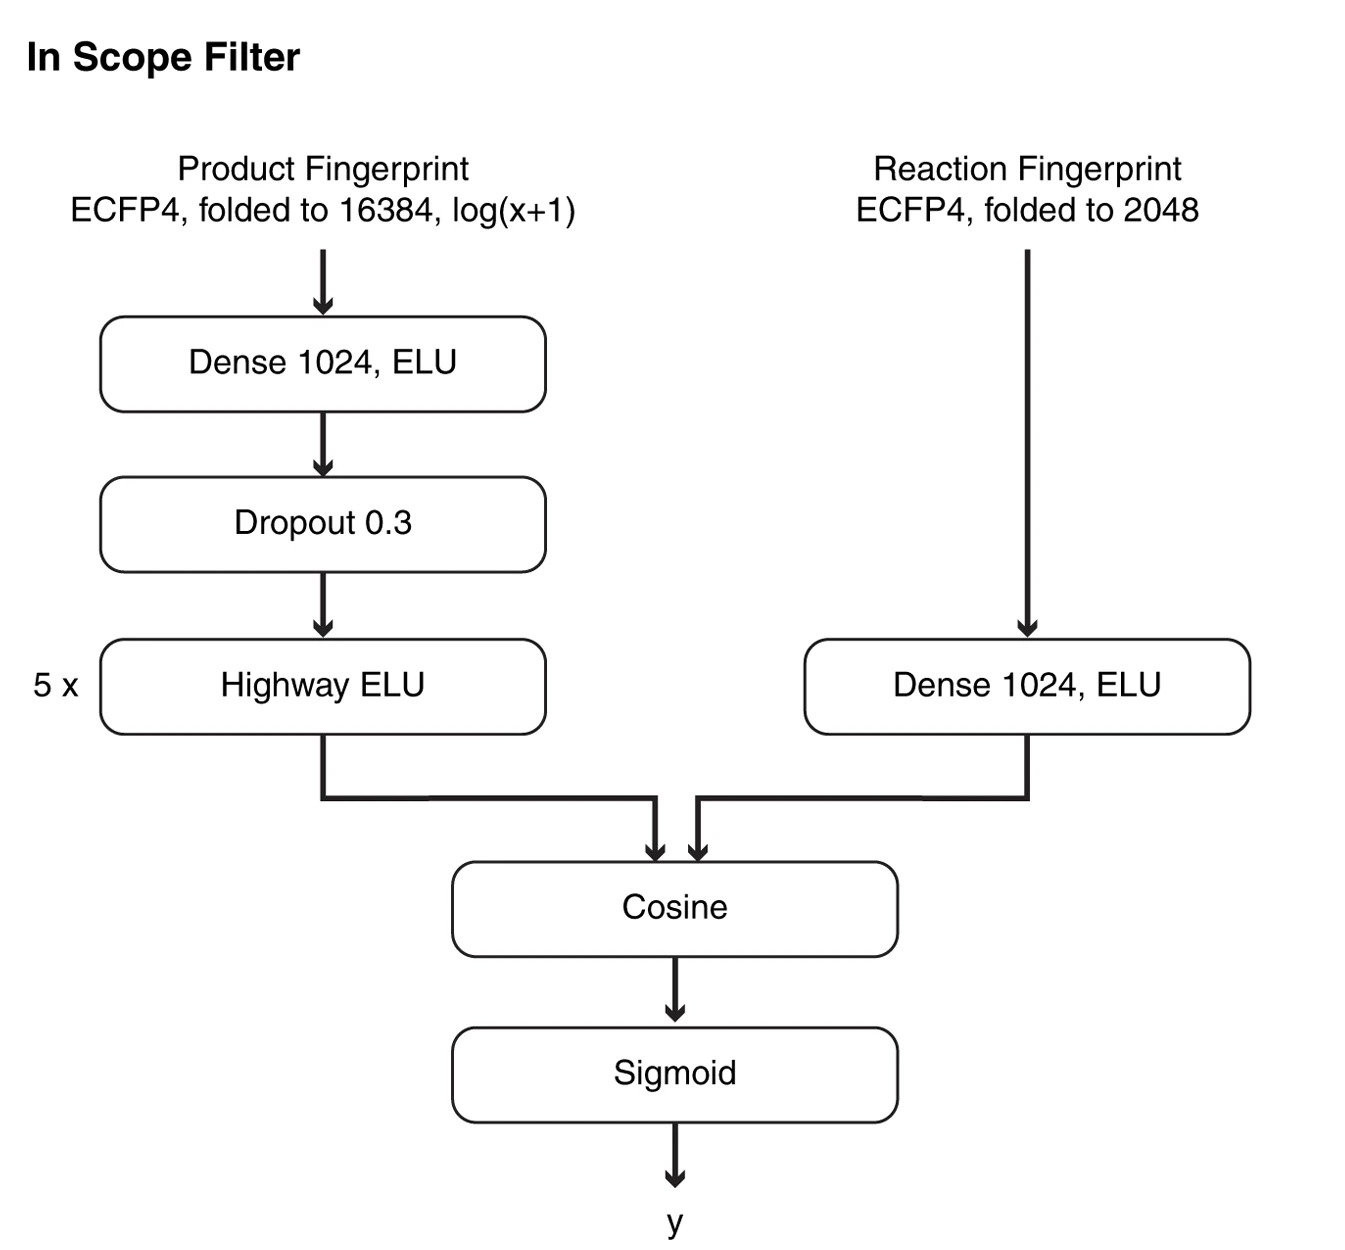
\includegraphics[]{in-scope-filter.jpg}
    \caption{Kuvassa In scope filter -neuroverkon rakenne.}
    {~\cite{SeglerMarwinHS2018Pcsw}}
\end{figure}

% IFN on neuroverkko, joka tarkistaa, onko EPN:än ja RPN:än valitsemat reaktiosäännöt toteutettavissa.

3N-MCTS:ässä IFN toimii binääriluokittelijana.
IFN kertoo, onko sille annettu yhdiste mahdollista muodostaa annetulla muunnossäännöllä.

IFN -neuroverkko muodostuu kahdesta haarasta.
Toinen haara saa syötteenä muodostettavan yhdisteen tunnisteen ja toinen haara saa muunnossäännön tunnisteen.

Haara, joka saa syöteenä yhdisteen tunnisteen, muodostuu yhdestä täysin kytketystä tasosta jonka jälkeen suoritetaan 0.3 dropout.
Tämän jälkeen data kulkee viiden highway -tason läpi.
Sekä täysin kytketty että highway -tasot käyttävät ELU -funktiota aktivointifunktiona.

Haara, joka saa syötteenään muunnossäännön tunnisteen, muodostuu vain yhdestä täysin kytketystä tasosta.
Tämä taso käyttää myös ELU -aktivointifuktiota.

Näiden haarojen jälkeen saaduista tuloksista lasketaan niiden kosinisamankaltaisuus.
Saatu tulos syötetään sitten sigmoid -funktiolle, jonka tulos kertoo, pystyykö kyseinen muunnosssäntö muodostamaan halutun yhdisteen.

IFN koulutetaan sekä onnistuneiden että epäonnistuiden sääntöjen avulla.
Koska epäonnistuneita sääntöjä ei tallenneta tietokantaan, niin kyseinen data generoidaan.
Data generoidaan siten, että jos reaktiossa \[A + B \rightarrow C\] lähtöaineet A ja B muodostavat reaktiossa lopputuotteen C, niin lopputuotteita D, E, F, jne.\@ ei muodostu (voisi selittää syvemmin).
IFN kouluttamista varten luotiin 100 miljoonaa epäonnistunutta reaktiota ja 10 miljoonaa epäonnistunutta reaktiota luotiin testaamista varten.

\subsubsection{3N-MCTS suorituskyky}

3N-MCTS -mallin suorituskykyä verrattiin BFS -menetelmään (Best-first search -method), joka käyttää heuristista käsinkoodattua \(SMILES^{3/2}\) -kustannefunktiota.
Tämä funktio antaa parhaimman tuloksen muunnossäännölle, joka jakaa halutun yhdisteen mahdollisimman hyvin yhtä suuriin lähtötuotteisiin.
Tästä menetelmästä luotiin myös versio, joka käyttää muokattua \(SMILES^{3/2}\) -kustannefunktiota.
Muokattu funktio käyttää 3N-MCTS:än expansion policy -neuroverkkoa ja in-scope filter -neuroverkkoa parhaimman muunnossäänön selvittämiseksi.

Mallit koulutettiin samoilla muunnossäännöillä ja testeissä käytettiin samaa aikaan perustuvaa jakoa.
Mallit koulutettiin muunnossäännöillä, jotka ilmenivät ennen vuotta 2015, ja malleja testatiin vuoden 2015 jälkeen ilmenneillä muunnossäänöillä.

Mallien tehtäväksi annettiin löytää halutulle yhdisteelle retrosyntetisointipolku annetussa ajassa.
Testaamiseen käytettiin 497 eri yhdistettä.

3N-MCTS suoriutui kahta muuta algoritmia paremmin jokaisessa eri aikakategoriassa.
3N-MCTS löysi viidessä sekunnissa 80 prosentille yhdisteistä retrosyntetisointipolun, kun taas muokattu \(SMILES^{3/2}\) -menetelmä löysi retrosyntetisointipolun vain 40 prosenttia yhdisteistä ja alkuperäinen ei löytänyt polkuja ollenkaan.
Kun aikaa kasvatettiin 60 sekunttiin per yhdiste, 3N-MCTS löysin 92 prosentille yhdisteistä polun, muokattu \(SMILES^{3/2}\) löysi 71 prosentille yhdisteistä ja alkuperäinen versio vain 4 prosentille yhdisteistä.

\begin{figure}
    \centering
    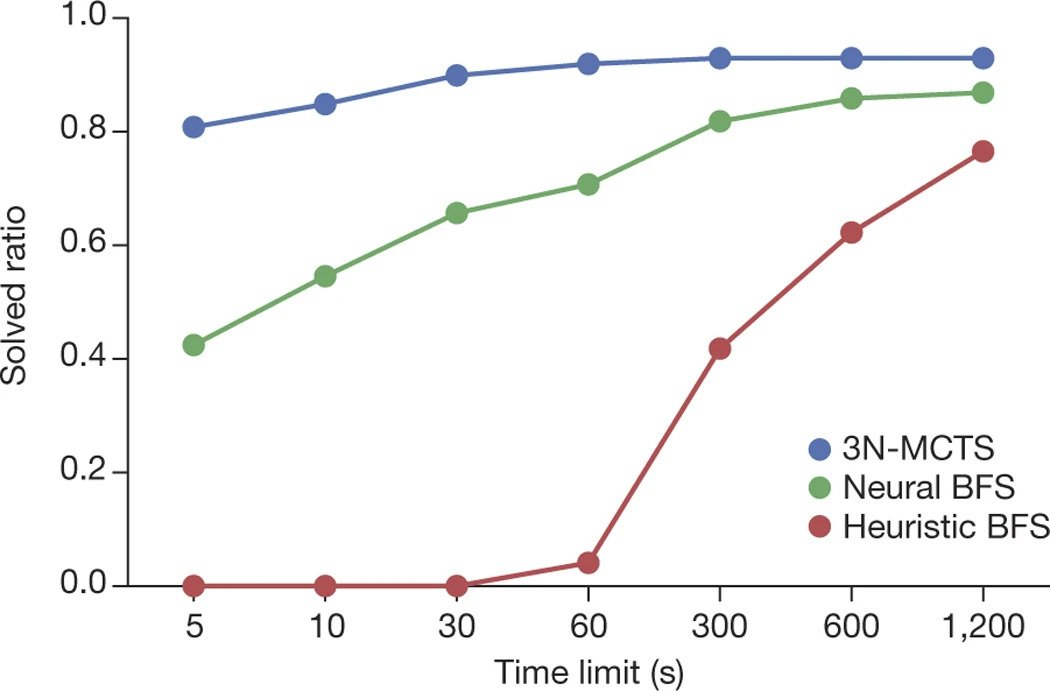
\includegraphics[width=8cm, height=6cm]{3N-MCTS-performance-fig.jpg}
    \caption{
        3N-MCTS:än suorituskyky verrattuna \(SMILES^{3/2}\) hyödyntävään BFS -menetelmään ja 3N-MCTS:än neuroverkkoja hyödyntävään BFS -menetelmään.
        Kuvaaja kertoo, kuinka monelle prosenttia annetuista yhdisteistä menetelmä kykenee löytämään retrosyntetisointipolun annaetusssa ajassa.
        Annetulla ajalla tarkoitetaan aikaa, jonka menetelmä voi korkeintaan käyttää yhden yhdisteen retrosyntetisointipolun löytämiseen.
    }
    {~\cite{SeglerMarwinHS2018Pcsw}}
\end{figure}

3N-MCTS:ää testattiin myös sokkotestillä 45 yliopistotason kemistille.
Testin tarkoituksena oli selvittää, suosivatko henkilöt ennemmin kirjallisuuteen perustuvaa retrosyntetisointipolkua vai 3N-MCTS:än antamaa polkua.
Sokkotestissä 57 prosenttia henkilöistä valitsi 3N-MCTS muodostaman polun ja loput valitsivat kirjallisuuteen perustuvan polun.


\subsection{Heurustiikka avusteiset neuroverkot}

On myös yleistä, että retrosynteesipolkuja suunnitelevat mallit hyödyntävät heurustiikka~\cite{ExpertKnowledgeRetorsynthesis}.
Badowski et al.\ ryhmä on kehittänyt koneoppimismallin, joka suunnittelee retrosynteesipolkuja hyödyntämällä neuroverkkoja ja ammattikemistien muodostamia heuristisia sääntöjä suunnitellessaan retrosynteesipolkua.

ICHO:n (Instytut Chemii Organicznej) kouluttamiseen käyettiin dataa 1.4 miljoonasta reaktiosta ja niiden lopputuotteista.
Data saadaan julkaistuista artikkeleista ja patenteista.
Reaktiolta kuitenkin vaaditaan, että ainakin yksi reaktio per lopputuote löytyy myös Chematican (taustatietoa) expert-coded säännöstöstä.
Lisäksi datasta suodatettiin pois suojaryhmien säännöt.

ICHO:sta kehitettiin myös malli, jonka kouluttamisessa käytettiin lisäksi vektoreita, jotka sisälsivät dataa kemiallisesti intuitiivisistä reaktiopiirteistä, joita on käytetty aikaisemmissa tutkimuksissa.
Tätä mallia kutsutaan ICHO+ malliksi, ja sitä käytetään vertailemaan ICHO mallin suoriutumista.

Kehitetyssä ICHO mallissa on kaksi tärkeää asiaa.

(1) Se laskee reaktioiden ilmaantumistodennäköisyyttä uudelleen perustaen kuinka usein ne ilmaantuvat ammattilaisten käyttämissä reaktioissa.
Tämä laskenta tapahtuu mallin koulutusvaiheessa.
Käytännössä tämä tarkoittaa, että koulutusvaiheessa mallilla on tieto, kuinka monta kertaa tietty reaktiosääntö ilmeni datassa ja kuinka monta kertaa kyseistä reaktiota käytettiin luomaan jokin lopputuote.
Malli laskee näiden välisen suhteen, jolloin se pystyy määrittämään, kuinka usein kyseistä reaktiota kannattaa käyttää.
Jos esimerkiksi jokin reaktio on mainittu datassa kymmenen kertaa ja samassa datassa kyseistä reaktiota käytetään kymmenen kertaa luomaan jokin lopputuote, niin malli käyttää tätä reaktiota, koska se luokitellaan `Helpoksi ja varmaksi toteuttaa'.
Jos suhde taas on pieni, niin reaktio luokitellaan `vaikeaksi toteuttaa'.

(2) Toiseksi se kykenee antamaan suuremman kuin nollatodennäköisyyden reaktiolle, joka ei ilmaantunut koulutusvaiheessa.
Tämä sen takia, että mallille koulutetaan jatkuva funktio, joka antaa todennäköisyyden jokaiselle reaktiotyypille perustuen, kuinka reaktio muuttaa lopputuotteen lähtötuotteiksi.
Eli jos jokin reaktion sormenjälki (Lisää tietoa, koska useassa mallissa käytetään) tai heuristinen kuvaus on samankaltainen toisen reaktion kanssa, joka ilmenee koulutusdatassa, niin reaktiolle voidaan antaa todennäköisyys sen käytölle.

\begin{figure}
    \centering
    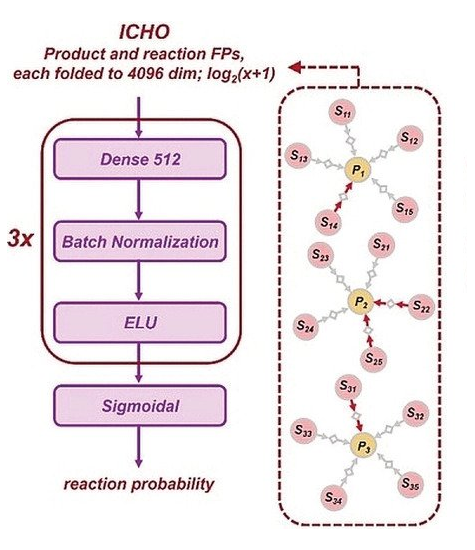
\includegraphics[width=8cm, height=8cm]{icho-neuralnetwork.png}
    \caption{ICHO -neuroverkon rakenne.}
    {~\cite{ExpertKnowledgeRetorsynthesis}}
\end{figure}

ICHO -malli muodostuu neljästä kerroksesta, joista kolme kerrosta ovat täysin kytkettyjä neuroverkkoja ja viimeinen taso on sigmoid -taso.
Samalla tavalla kuin 3N-MCTS mallissa, ICHO -malli käyttää myös ELU -aktivointifunktiota.
ICHO -malli käyttää Batch normaliztion -algoritmia koulutusvaiheessa.
Batch normalization -algoritmin idea on standardoida koulutusvaiheessa kerrokselle tuleva syöte, jolla verkon painoja muutetaan.

ICHO mallia vertailtiin aikasiemmin mainitun 3N-MCTS -mallin kanssa, jota kustsutaan artikkelissa SW mallina.
Kyseisestä SW mallista kehitettiin myös heuristista dataa hyödyntävä malli SW+.
Lisäksi luotiin SW malli, joka ei käy läpi kaikkia mahdollisia reaktioita, vaan valitsee säännöt niistä reaktioista, jotka eivät aiheuta konfliktia (selitys) ja jotka johtavat vain tiettyyn lopputuotteeseen.
Tätä mallia kutsutaan SW2 -malliksi ja tästä luodusta heuristisesta mallista käytetään nimeä SW2+.
Lisäksi vertailumalliksi luodaan täysin heuristinen malli, joka arvioi reaktioita sen mukaan, kuinka paljon ne rakenteellisesti yksinkertaistavat lopputuotetta.
Tämä malli suosii reaktioita, jotka pilkkovat molekyylin keskeltä, eli puolittavat sen.
Tämä on haluttu lähestymistapa retrosynteesiin, koska se minimoi syntetisointivaiheiden määrän.

\subsubsection{ICHO suorituskyky}

ICHO -mallia testataan eri tavalla 3N-MCTS mallia, jossa mitataan, kuinka monelle yhdisteelle malli kykenee löytämään toimivan retrosyntetisointipolun tietyssä ajassa.
ICHO -mallia testataan siten, että jokaiselle mallille annetaan yhdiste, ja malli antaa tulosteena listan muunnossäännöistä, jotka on asetettu paremmuusjärjestykseen niille annetun pisteytyksen mukaan.
Muunnossäänön pisteytys kertoo, kuinka paljon malli suosittelee käytettävän kyseistä muunnossääntöä.
Näistä muunnossäännöistä laskettiin, kuinka suuri osa niistä pohjautuu johonkin aikaisempaan muunnossääntöön, joka on esiintynyt kirjallisuudessa tai patenteissa.
Mitä suurempi osa ehdotetuista muunnossäänöistä löytyy kirjallisuudesta, sitä paremmin malli toimii.

Miten koneoppimista hyödynnetään tällä hetkellä lääkkeiden syntetisoinnissa~\cite{SeglerMarwinHS2018Pcsw,ShaharHarelAndKiraRadinsky,ShinBonggun}?

\chapter{Lääkkeiden kehitys tulevaisuudessa}

Vaikka koneoppimisen käyttökohteet ovat yleistyneet lääkekehityksessä, niin koneoppimisen lähestymistavoilla on edelleen potenttiaalia kehittyä~\cite{ButlerKeithT2018Mlfm}.

Yksi kehityksen kohteista on tehokkaampi datan tulkinta pienestä aineistomäärästä.
Paikoin kemian ja lääkekehityksen alalla on muihin koneoppimismallien käyttökohteisiin verrattaen vähän dataa saatavilla ja sitä on kallista tuottaa.
Tämä vaatii tutkijoilta enemmän työtä, jotta tieteellisistä julkaisuista saatava data saadaan koneiden hyödyntämään muotoon.
Toinen ratkaisu tähän on meta-oppimis (selitys) lähestymistapa.
Uudet lähestymistavat kuten Neuro Turing kone ja matkija oppiminen mahdollistavatkin oppimisen vähästä määrästä dataa ja Bayes luokittelija on suoriutunut lähes ihmistasoisesti käyttämällä One-shot oppismallia.

Toinen merkittävä edistysaskel on kemiallisten yhdisteiden ja reaktioiden tehokkaampi esitysmalli.
Tähän asti kemiaa on esitetty ihmisten ymmärtämässä muodossa, mutta tämä ei aina ole koneelle paras esitysmalli.
Koneoppimismallit käyttävät tietoa molekyyleistä ja atomeista ja koneoppimismallit ovat niin hyviä kuin nämä kuvaukset.
Hyvältä kuvaukselta vaaditaan, että sen avulla on yksinkertaista hankkia kohteen ominaisuudet ja sen tulee olla mahdollisimman pieni ulotteinen.
Uusia kuvausmalleja on kehitetty ja koska uudet mallit ovat näyttäneet, että ne ovat tehokkaita, niin uusien kuvauksien kehittäminen jatkuu edelleen.

Kemiallista koneoppimista edistävä asia on myös kvanttilaskennan hyödyntäminen.
Kvanttikoneiden suuri laskuteho pystyy vähentämään uusien mallien koulutusaikaa merkittävästi.

Koenoppimista voidaan mahdollisesti käyttää tulevaisuudessa uusien tieteellisten lakien löytämisessä.
Mutta vaikka eri koneoppimisesta kehitetyt mallit ovat ennalta arvattavia, niin ne eivät kuitenkaan ole aina tulkittavia.
Neuroverkko voi esimerkiksi oppia ideaalin kaasulain \((pV=nRT)\), mutta neuroverkon kaarien painojen muuttaminen ymmärrettäväksi säännöksi ei ole yksinkertainen tehtävä.
Voi olla, että koneoppimismalli pystyy huomaamaan datasta säännön, joka toistuu, mutta jos tutkijat eivät tiedä tai tunne kyseistä sääntöä, niin mallin tulkitseminen on lähes mahdotonta.

\chapter{Yhteenveto}

\cleardoublepage{}                          %fixes the position of bibliography in bookmarks
\phantomsection{}
\addcontentsline{toc}{chapter}{\bibname}  % This lines adds the bibliography to the ToC
\printbibliography{}

%%%%%%%%%%%%%%%%%%%%%%%%%%%%%%%%%%%%%%%%%%%%%%%%%%%%%%%%%
\backmatter{}
% \begin{appendices}

%     \appendix{Sample Appendix\label{appendix:model}}
%     usually starts on its own page, with the name and number of the appendix at the top.
%     The appendices here are just models of the table of contents and the presentation. Each appendix
%     Each appendix is paginated separately.

%     In addition to complementing the main document, each appendix is also its own, independent entity.
%     This means that an appendix cannot be just an image or a piece of programming, but the appendix must explain its contents and meaning.

% \end{appendices}
%%%%%%%%%%%%%%%%%%%%%%%%%%%%%%%%%%%%%%%%%%%%%%%%%%%%%%%%%

\end{document}
